\chapter{Impact of TOF on Respiratory Motion Model Estimation Using NAC PET} \label{sec:impact_of_tof_on_respiratory_motion_model_estimation_using_nac_pet}
    \newpage
    
    \longsection{Introduction}{sec:impact_of_tof_on_respiratory_motion_model_estimation_using_nac_pet_introduction}
        This chapter of the thesis contains the work performed in the domain of \gls{MC}. The first section of this chapter introduces preliminary work on the feasibility of \gls{MC} when \gls{AC} is not applied both with and without \gls{TOF}.
        
        The second section of this chapter highlights further work to incorporate \gls{AC} into the work from the first section. Here methods to warp a single \gls{CT} derived \gls{Mu-Map} to position at each gate using a \gls{MM} are introduced. In addition, the advantage of fitting a further \gls{MM} on the newly \gls{AC} data will be evaluated.
        
        The third section of this chapter introduces a comparison between different \gls{MC} methods, both with and without \glss{MM}. Here the data used is of very low count with a \gls{Mu-Map} at end inhalation (close to a breath hold \gls{Mu-Map}).
        
        Finally, the fourth section of this chapter discusses the problems or limitations of the work performed in the previous two sections, including some possible directions in which to rectify these limitations as well as specifying where future work may take place.
    
    
    \longsection{Impact of TOF on Respiratory Motion Model Estimation Using Pre-Gated No Intra-Cycle Motion NAC PET}{sec:impact_of_tof_on_respiratory_motion_model_estimation_using_pre_gated_no_intra_cycle_motion_nac_pet}
        This section investigates the possibility of using \glss{MM} for respiratory \gls{MC} in \gls{PET}/\gls{CT}, and in particular whether incorporating \gls{TOF} information increases the accuracy of the \glss{MM} derived from \gls{NAC} reconstructed images.
        
        \subsection{Introduction} \label{sec:impact_of_tof_on_respiratory_motion_model_estimation_using_pre_gated_no_intra_cycle_motion_nac_pet_introduction}
        As discussed in~\Fref{sec:motion_modelling}, \gls{RM} reduces image quality in \gls{PET} by causing artefacts and loss of resolution in the thoracic region~\boxcite{Nehmeh2008a}. Many methods have been proposed to correct for \gls{RM}, usually involving registration between a reference volume and a set of volumes in different positions in the respiratory cycle obtained by gating~\boxcite{Oliveira2014}. However, such pair wise registration is sensitive to noise. It also does not allow prediction of the respiratory state for data not used to estimate the motion, for instance, to be used for real time \gls{MC}. \gls{SS} driven \glss{MM} attempt to overcome these deficiencies by relating the motion in the data to a number of \gls{SS} values~\boxcite{McClelland2013}. The model can output a transformation or \gls{DVF} for every value of a \gls{SS}. \glss{MM} are fit on a series of either time or gating based volumes.

        To avoid mis-registration due to attenuation mismatches, most existing methods rely on pair wise registration of \gls{NAC} \gls{PET} volumes. The benefits of using \gls{AC} \gls{PET} for \gls{IR} are unclear. If images are reconstructed using a static \gls{Mu-Map}, then artefacts caused by the misalignment between the activity distribution and the \gls{Mu-Map} would hamper \gls{IR}. It could therefore be advantageous to estimate motion on \gls{NAC} images~\boxcite{LungMotionDiaphragmBaiBib}~\boxcite{Kalantari2017AttenuationRegistration:}~\boxcite{Dawood2008RespiratoryAlgorithms}~\boxcite{Dawood2006LungImages}. However, this is a challenging problem due to the low contrast and high noise of these volumes. Contrast may be too low to fit an accurate \gls{MM} and artefacts associated with the mismatch between the acquisition data and \gls{Mu-Map} could also obscure the underlying motion if \gls{AC} is used.
        
        In the absence of \gls{TOF}, there is no information on the activity position along the \gls{LOR} and \gls{NAC} reconstructions have high intensity near the surface and low contrast in the internal part of the body. In \gls{TOF}, the time information constrains the activity position along the \gls{LOR} changing the nature and extent of the artefacts associated with \gls{NAC} \gls{PET} as well as changing noise properties~\boxcite{Ter-Pogossian1981}.
        
        The aim of this section is to investigate whether \gls{TOF} can sufficiently increase the contrast and lower the noise of \gls{NAC} images to facilitate the calculation of accurate \glss{MM}.
        
        \subsection{Methods} \label{sec:impact_of_tof_on_respiratory_motion_model_estimation_using_pre_gated_no_intra_cycle_motion_nac_pet_methods}
            \subsubsection{XCAT Image Generation} \label{sec:impact_of_tof_on_respiratory_motion_model_estimation_using_pre_gated_no_intra_cycle_motion_nac_pet_methods_xcat_image_generation}
                \gls{XCAT}~\boxcite{Segars2010} was used to generate six volumes over a \SI{5.0}{\second} second breathing cycle, as discussed in~\Fref{sec:respiratory_correspondence_model}, with one volume at full expiration at the beginning of the cycle and one volume at full expiration at the end of the cycle and using the default \gls{XCAT} settings for the extent of \gls{AP} and \gls{SI} motion (default \gls{XCAT} settings being a single orthodox breathing trace). The default \gls{XCAT} settings being a, peak to peak, \SI{2.0}{\centi\metre} \gls{RM} displacement over \SI{5.0}{\second}. Activity concentrations were derived from a static \gls{18F-FDG} patient scan. The \gls{FOV} included the base of the lungs, diaphragm and the top of the liver with a \SI{40.0}{\milli\metre} diameter spherical lesion placed in the right lung.
            
            \subsubsection{PET Data Simulation} \label{sec:impact_of_tof_on_respiratory_motion_model_estimation_using_pre_gated_no_intra_cycle_motion_nac_pet_methods_pet_data_simulation}
                \gls{PET} acquisitions were simulated using \gls{STIR}~\boxcite{Thielemans2012} through \gls{SIRF}~\boxcite{Ovtchinnikov2017} to forward project the input data to sinograms using the geometry of a \gls{GE} Discovery 690/710 and, where relevant, a \gls{TOF} resolution of \SI{375.0}{\pico\second} similar to the \gls{GE} Signa \gls{PET}/\gls{MR} (using \gls{TOF} mashing to reduce computation time resulting in $13$ \gls{TOF} time bins of size \SI{376.5}{\pico\second}). Attenuation was included in the simulation using the relevant \gls{Mu-Map} generated by \gls{XCAT}. Scatter and randoms were not taken into account in the simulation. Poisson noise realisations were generated to simulate an acquisition as if it had been gated into six bins over an acquisition of \SI{120}{\second}, emulating a standard single bed position acquisition. 
            
            \subsubsection{Image Reconstruction} \label{sec:impact_of_tof_on_respiratory_motion_model_estimation_using_pre_gated_no_intra_cycle_motion_nac_pet_methods_image_reconstruction}
                Data were reconstructed without \gls{AC} using \gls{OSEM} with two full iterations and $24$ subsets~\boxcite{Hudson1994}. Volumes were post filtered using a \gls{3D} Gaussian blurring with a kernel size of \SI{6.4}{\milli\metre} \gls{FWHM}.
            
            \subsubsection{Motion Model Estimation} \label{sec:impact_of_tof_on_respiratory_motion_model_estimation_using_pre_gated_no_intra_cycle_motion_nac_pet_methods_motion_model_estimation}
                Following on from what is presented in~\Fref{sec:respiratory_correspondence_model} a generalised framework unifying registration and \gls{MM} estimation, NiftyRegResp, was used to estimate the \gls{RCM}. \glss{RCM} being the models fit on the acquired \gls{SS} and \glss{DVF} which, as a function can, take in a \gls{SS} value and return the \gls{DVF} which can be used to warp a volume to a reference position. Here, using \gls{SSD} as the objective function~\boxcite{McClelland2017}.
                
            \subsubsection{Evaluation} \label{sec:impact_of_tof_on_respiratory_motion_model_estimation_using_pre_gated_no_intra_cycle_motion_nac_pet_methods_evaluation}
                Three \glss{RCM} were compared: calculated from the \gls{PET} \gls{XCAT} volumes (gold standard), \gls{NTOF} \gls{NAC} reconstructions and \gls{TOF} \gls{NAC} reconstructions. To test the accuracy of the \glss{RCM}, the three models were used to warp the \gls{PET} volume generated by \gls{XCAT} at the mean breathing position, to the position at each gate. The mean breathing position \gls{XCAT} volume was generated by calculating the mean \gls{SS} value and using this as an input to \gls{XCAT}. A mean position volume was used as the \gls{RCM} was fit with this as the reference position for the \gls{SS}, as discussed in~\Fref{sec:motion_modelling}. These estimated volumes were then compared to the original \gls{XCAT} input volumes. Difference volumes were obtained by subtracting the original \gls{XCAT} volume $\mathbf{f}_t$ and warped volumes $\mathbf{W}(\alpha_t) \mathbf{f}_\mathrm{ref}$ at the same gate. \gls{MAPE} were computed from these difference images. \gls{MAPE} is expressed as:
                
                \begin{equation} \label{eq:impact_of_tof_on_respiratory_motion_model_estimation_using_pre_gated_no_intra_cycle_motion_nac_pet_methods_mape}
                   M := \frac{\frac{1}{n}\sum_{n}\mid e_n - g_n \mid}{\frac{1}{n}\sum_{n}g_n} \times 100
                \end{equation}
                
                \noindent where in~\Fref{eq:impact_of_tof_on_respiratory_motion_model_estimation_using_pre_gated_no_intra_cycle_motion_nac_pet_methods_mape} $n$ is the number of volumes, $e_n$ are the estimated volumes and $g_n$ are the \gls{GT} volumes.
                
                In addition, the \gls{COM} of the lesion was also tracked over the six gates, by warping a volume only including the lesion in the reference position as above, and then computing the \gls{COM}. The \gls{COM} along each dimension is calculated using the following equation:
                
                \begin{equation} \label{eq:impact_of_tof_on_respiratory_motion_model_estimation_using_pre_gated_no_intra_cycle_motion_nac_pet_methods_com}
                   C_{d} := \frac{1}{n}\sum_{i = 1}^{n} d_{i}
                \end{equation}
                
                \noindent where in~\Fref{eq:impact_of_tof_on_respiratory_motion_model_estimation_using_pre_gated_no_intra_cycle_motion_nac_pet_methods_com} $n$ is the number of distinct points along dimension $d_1 \dotso d_n$.
            
        \subsection{Results} \label{sec:impact_of_tof_on_respiratory_motion_model_estimation_using_pre_gated_no_intra_cycle_motion_nac_pet_results}
            \begin{figure}
                \centering
                
                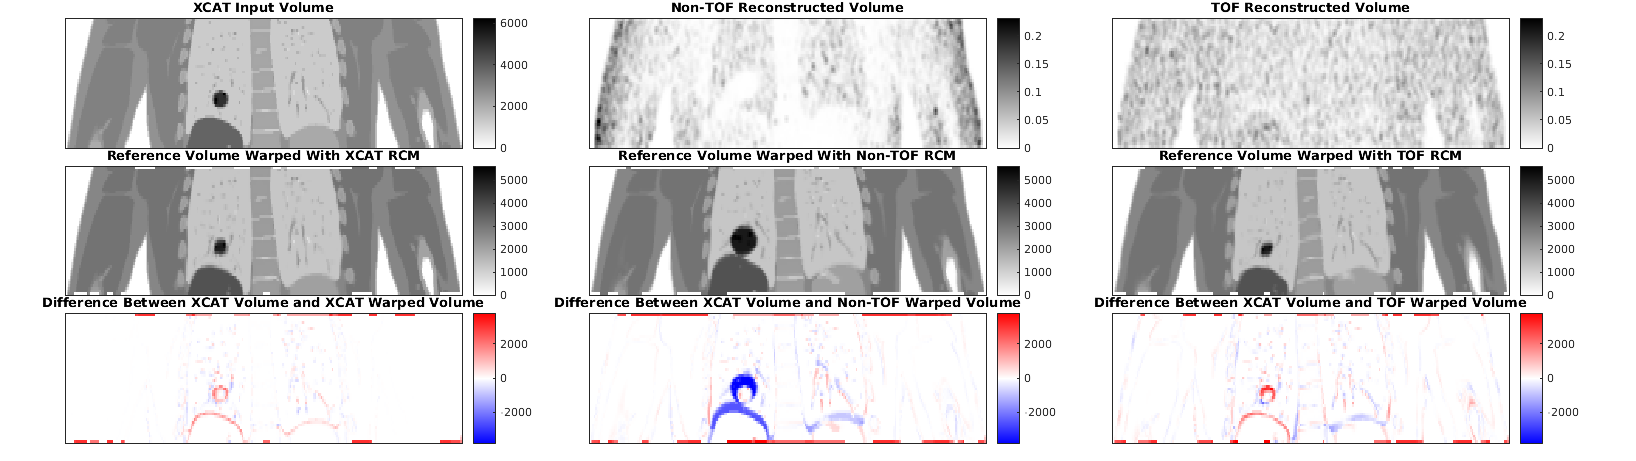
\includegraphics[width=1.0\linewidth]{figures/motion_correction_results_1_output.png}
                
                \captionsetup{singlelinecheck=false, justification=raggedright}
                \caption{All volumes correspond to end inhalation. First row from left to right: \gls{XCAT} \gls{PET} data, \gls{NAC} \gls{NTOF} reconstructed data and \gls{NAC} \gls{TOF} reconstructed data. Second row: \glss{RCM} applied to mean position \gls{XCAT} data with \glss{RCM} derived from \gls{XCAT} \gls{PET} data (left), \gls{NAC} \gls{NTOF} (middle) and \gls{NAC} \gls{TOF} (right) volumes. Colour map ranges are consistent for all images on this row. The third row from left to right:  difference between the estimated volumes from the second row with the \gls{XCAT} end inhalation volume. Colour map ranges are consistent for all images on this row.} \label{fig:impact_of_tof_on_respiratory_motion_model_estimation_using_pre_gated_no_intra_cycle_motion_nac_pet_results_output}
            \end{figure}
            
            \begin{table}
                \centering
                
                \captionsetup{singlelinecheck=false, justification=raggedright}
                \caption{Comparison of the \gls{MAPE} between the \gls{GT} data and the volumes estimated from the \gls{XCAT} based \glss{RCM}, the volumes estimated from the \gls{NAC} \gls{NTOF} based \gls{RCM} and the volumes estimated from the \gls{NAC} \gls{TOF} based \gls{RCM}.}
                
                \resizebox*{1.0\linewidth}{!}
                {
                    \begin{tabular}{||c|ccc||}
                        \hline
                        \textbf{\gls{MAPE}} & \textbf{XCAT} & \textbf{\gls{NTOF}} & \textbf{\gls{TOF}} \\
                        \hline
                        \textbf{$1$} & $1.95$ & $8.35$ & $4.18$ \\
                        \textbf{$2$} & $1.59$ & $1.61$ & $1.84$ \\
                        \textbf{$3$} & $2.06$ & $9.91$ & $5.23$ \\
                        \textbf{$4$} & $1.97$ & $6.15$ & $3.68$ \\
                        \textbf{$5$} & $1.65$ & $4.45$ & $2.52$ \\
                        \textbf{$6$} & $1.95$ & $8.35$ & $4.18$ \\
                        \hline
                        \textbf{Mean} & $1.86$ & $6.47$ & $3.60$ \\
                        \hline
                    \end{tabular}
                } \label{tab:impact_of_tof_on_respiratory_motion_model_estimation_using_pre_gated_no_intra_cycle_motion_nac_pet_results_mape}
            \end{table}
            
            \begin{figure}
                \centering
                
                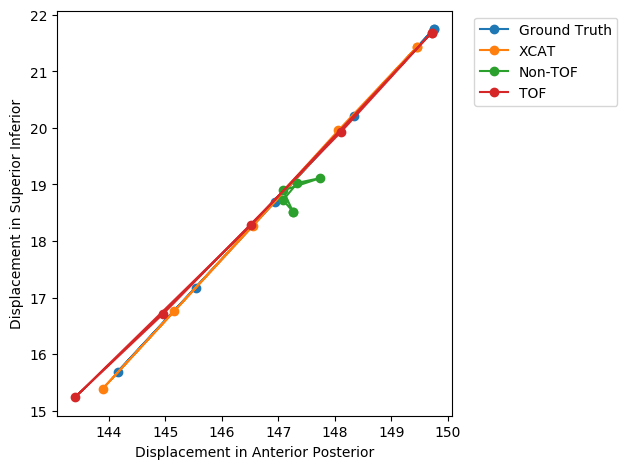
\includegraphics[width=1.0\linewidth]{figures/motion_correction_results_1_TOF.png}
                
                \captionsetup{singlelinecheck=false, justification=raggedright}
                \caption{The path of the \gls{COM} of the lesion, in voxel indices. Horizontal (respectively vertical) axis corresponds to motion in the \gls{AP} (respectively \gls{SI}) direction over the six gates. Different curves denote \gls{COM} displacement for \gls{GT} data, the estimated data from the \gls{XCAT} based \gls{RCM}, the estimated data from the \gls{NAC} \gls{NTOF} based \gls{RCM} and the estimated data from the \gls{NAC} \gls{TOF} based \gls{RCM}.} \label{fig:impact_of_tof_on_respiratory_motion_model_estimation_using_pre_gated_no_intra_cycle_motion_nac_pet_results_com_graph}
            \end{figure}
            
             The reconstructed data, estimated volumes and difference can be seen in~\Fref{fig:impact_of_tof_on_respiratory_motion_model_estimation_using_pre_gated_no_intra_cycle_motion_nac_pet_results_output} and \gls{MAPE} are in~\Fref{tab:impact_of_tof_on_respiratory_motion_model_estimation_using_pre_gated_no_intra_cycle_motion_nac_pet_results_mape}. The mean \gls{MAPE} was found to be lower for the \gls{NAC} \gls{TOF} data than for the \gls{NAC} \gls{NTOF}.
            
             \gls{COM} results can be seen in~\Fref{fig:impact_of_tof_on_respiratory_motion_model_estimation_using_pre_gated_no_intra_cycle_motion_nac_pet_results_com_graph}. The path of the \gls{NAC} \gls{TOF} data follows the \gls{GT} path much closer than the \gls{NAC} \gls{NTOF} data, and is quite close to the gold standard \gls{XCAT}-derived motion.
            
        \subsection{Conclusion} \label{sec:impact_of_tof_on_respiratory_motion_model_estimation_using_pre_gated_no_intra_cycle_motion_nac_pet_conclusion}
            \glss{MM} derived from \gls{NAC} \gls{TOF} volumes were found to be more robust than when using \gls{NAC} \gls{NTOF}, both visually and when comparing \gls{MAPE} and \gls{COM}. This was noticeable for the lung lesion in the thoracic cavity but also for other parts of the anatomy such as the liver. This is likely due to the improved image contrast of \gls{NAC} \gls{TOF} images.

            In the future, research will focus on investigating the robustness of the \gls{MM} estimation to different noise levels, acquisition duration and size of lesion. This will be expanded upon in~\Fref{sec:impact_of_tof_on_respiratory_motion_model_estimation_using_nac_pet_discussion}.
    
    \longsection{PET/CT Respiratory Motion Correction With a Single Attenuation Map Using NAC Derived Deformation Fields}{sec:pet_ct_respiratory_motion_correction_with_a_single_attenuation_map_using_nac_derived_deformation_fields}
        This section investigates the possibility of using \gls{MM} for inter-respiratory cycle \gls{MC} in \gls{PET}/\gls{CT}, and in particular whether iterative estimation of both the motion parameters and warping of a single \gls{Mu-Map}, from any respiratory position, increases the accuracy of \gls{AC} reconstruction.
        
        \subsection{Introduction} \label{sec:pet_ct_respiratory_motion_correction_with_a_single_attenuation_map_using_nac_derived_deformation_fields_introduction}
            Following on from what was presented in~\Fref{sec:impact_of_tof_on_respiratory_motion_model_estimation_using_pre_gated_no_intra_cycle_motion_nac_pet_introduction} additionally there are different strategies for handling \gls{AC} in conjunction with \gls{MC} exist. In clinical practice, usually a single \gls{Mu-Map} is available, derived from \gls{CT} in one respiratory state. This can introduce an unwanted bias (through misaligned anatomy) into the \gls{MC} algorithm. Other \gls{MC} methods can incorporate, directly, both \gls{MC} and \glss{Mu-Map} estimation into reconstruction, however, these can be computationally expensive~\boxcite{Bousse2016b}.
            
            This section builds upon previous work, presented in~\Fref{sec:impact_of_tof_on_respiratory_motion_model_estimation_using_pre_gated_no_intra_cycle_motion_nac_pet_methods} and evaluated in~\Fref{sec:impact_of_tof_on_respiratory_motion_model_estimation_using_pre_gated_no_intra_cycle_motion_nac_pet_results}, which suggested that \gls{NAC} data was suitable for motion estimation, through the use of \glss{MM}, if \gls{TOF} data are available. Here, the previous work is expanded upon by incorporating \gls{AC} in an iterative process. In our previous work, seen here in~\Fref{sec:impact_of_tof_on_respiratory_motion_model_estimation_using_pre_gated_no_intra_cycle_motion_nac_pet_introduction}, we investigated the possibility of using a \gls{MM} for respiratory \gls{MC} where the \gls{MM} was derived from \gls{NAC} \gls{PET}. We found that \gls{NAC} \gls{TOF} \gls{PET} was suitable to estimate the motion from gated \gls{PET} data without inter-respiratory cycle variation~\boxcite{Whitehead2019ImpactPET}. This work extends the method towards \gls{AC} with a single \gls{Mu-Map} (from any position).
        
        \subsection{Methods} \label{sec:pet_ct_respiratory_motion_correction_with_a_single_attenuation_map_using_nac_derived_deformation_fields_methods}
            \gls{NAC} are reconstructed using \gls{OSEM}, seen in~\Fref{sec:pet_ct_respiratory_motion_correction_with_a_single_attenuation_map_using_nac_derived_deformation_fields_methods_xcat_volume_generation},~\Fref{sec:pet_ct_respiratory_motion_correction_with_a_single_attenuation_map_using_nac_derived_deformation_fields_methods_pet_acquisition_simulation} and~\Fref{sec:pet_ct_respiratory_motion_correction_with_a_single_attenuation_map_using_nac_derived_deformation_fields_methods_non-attenuation_corrected_image_reconstruction}, and used as input for \gls{MM} estimation, seen in~\Fref{sec:pet_ct_respiratory_motion_correction_with_a_single_attenuation_map_using_nac_derived_deformation_fields_methods_motion_model_estimation}. A single \gls{Mu-Map} is then warped to the volumes, using the \gls{MM}, the volumes are \gls{AC}, seen in~\Fref{sec:pet_ct_respiratory_motion_correction_with_a_single_attenuation_map_using_nac_derived_deformation_fields_methods_attenuation_map_warping}, after which another motion estimation and correction cycle is performed, seen in~\Fref{sec:pet_ct_respiratory_motion_correction_with_a_single_attenuation_map_using_nac_derived_deformation_fields_methods_attenuation_corrected_image_reconstruction}.
            
            For validation, \gls{XCAT} simulations are used, for one bed position, with a \gls{FOV} including the base of the lungs and the diaphragm. The output from the proposed method is evaluated against a \gls{NMC} reconstruction of the same data visually, using a profile as well as \gls{SUV} analysis, seen in~\Fref{sec:pet_ct_respiratory_motion_correction_with_a_single_attenuation_map_using_nac_derived_deformation_fields_methods_evaluation}.
            
            \subsection{XCAT Volume Generation} \label{sec:pet_ct_respiratory_motion_correction_with_a_single_attenuation_map_using_nac_derived_deformation_fields_methods_xcat_volume_generation}
                Volume generation follows the same basic structure as presented in~\Fref{sec:impact_of_tof_on_respiratory_motion_model_estimation_using_pre_gated_no_intra_cycle_motion_nac_pet_methods_xcat_image_generation}, however here $240$ volumes were generated over a \SI{120}{\second} respiratory trace (with inter-respiratory cycle variation) derived from data captured using a \gls{RPM}. The max displacement of \gls{AP} and \gls{SI} motion was set to \SI{1.2}{\centi\metre} and \SI{2.0}{\centi\metre} respectively. The \gls{FOV} included the base of the lungs, diaphragm and the top of the liver with a \SI{20}{\milli\metre} diameter spherical lesion placed into the centre of the right lung.
    
            \subsection{PET Acquisition Simulation} \label{sec:pet_ct_respiratory_motion_correction_with_a_single_attenuation_map_using_nac_derived_deformation_fields_methods_pet_acquisition_simulation}
                Again as in~\Fref{sec:impact_of_tof_on_respiratory_motion_model_estimation_using_pre_gated_no_intra_cycle_motion_nac_pet_methods_pet_data_simulation} \gls{PET} simulation (and reconstructed) followed the same basic structure, using \gls{STIR}~\boxcite{Thielemans2012}~\boxcite{Nikos2019}~\boxcite{Wadhwa2020PETLibrary} through the \gls{SIRF}~\boxcite{Ovtchinnikov2017}, to forward project data using the geometry of a \gls{GE} Discovery $710$, but using a \gls{TOF} resolution of \SI{375}{\pico\second}. This \gls{TOF} resolution is higher than that of the $710$, but is closer to the newer \gls{GE} Signa \gls{PET}/\gls{MR} system. \gls{TOF} mashing was used to reduce computation time resulting in $13$ \gls{TOF} bins of size \SI{376.5}{\pico\second}. Multiple noise realisations were generated to simulate an acquisition over \SI{120}{\second}, emulating a standard single bed position acquisition. A respiratory \gls{SS} was generated using \gls{PCA}~\boxcite{Thielemans2011}, for more information see~\Fref{sec:respiratory_signal_detection}. This was used to gate the data into $10$ respiratory bins using displacement gating. For the purpose of the \gls{MM} fitting, \gls{SS} values were ascertained for the post-gated data by taking an average of the \gls{SS} values of the data in each bin.
            
            \subsection{Non-Attenuation Corrected Image Reconstruction} \label{sec:pet_ct_respiratory_motion_correction_with_a_single_attenuation_map_using_nac_derived_deformation_fields_methods_non-attenuation_corrected_image_reconstruction}
                Data were reconstructed without \gls{AC} using \gls{OSEM} with two full iterations and $24$ subsets~\boxcite{Hudson1994}.
                Volumes were post-filtered using a \gls{3D} Gaussian blur with a kernel size of \SI{6.4}{\milli\metre} full width half maximum.
            
            \subsection{Motion Model Estimation} \label{sec:pet_ct_respiratory_motion_correction_with_a_single_attenuation_map_using_nac_derived_deformation_fields_methods_motion_model_estimation}
                Following on from what is presented in~\Fref{sec:respiratory_correspondence_model} and~\Fref{sec:impact_of_tof_on_respiratory_motion_model_estimation_using_pre_gated_no_intra_cycle_motion_nac_pet_methods_motion_model_estimation} a generalised framework unifying \gls{IR} and respiratory \glss{MM} were used to estimate \glss{MM} and \glss{MCI}~\boxcite{McClelland2017}. \gls{SSD} was used as the similarity measure and \gls{BE} was used as a penalty. The \gls{CPG} spacing and penalty weight were tuned using a grid search.
            
            \subsection{Attenuation Map Warping} \label{sec:pet_ct_respiratory_motion_correction_with_a_single_attenuation_map_using_nac_derived_deformation_fields_methods_attenuation_map_warping}
                A \gls{Mu-Map} close to the mean respiratory position was selected from the \glss{Mu-Map} generated by \gls{XCAT}. This \gls{Mu-Map} was then registered (using \gls{NMI}) to the mean position \gls{NAC} \gls*{MCI} generated using the \gls{MM}. The \gls{MM} was then used to generate \glss{DVF} for the \gls{SS} values of each bin, which were then used to warp the \gls{Mu-Map} from the mean respiratory position to each bin.
            
            \subsection{Motion Corrected Image Reconstruction with AC} \label{sec:pet_ct_respiratory_motion_correction_with_a_single_attenuation_map_using_nac_derived_deformation_fields_methods_attenuation_corrected_image_reconstruction}
                Data were re-reconstructed, with \gls{AC}, using the \glss{Mu-Map} from~\Fref{sec:pet_ct_respiratory_motion_correction_with_a_single_attenuation_map_using_nac_derived_deformation_fields_methods_attenuation_map_warping}. The same reconstruction parameters as in~\Fref{sec:pet_ct_respiratory_motion_correction_with_a_single_attenuation_map_using_nac_derived_deformation_fields_methods_attenuation_corrected_image_reconstruction} were used. These data were then either \gls{MC} using the original \gls{NAC} \gls{MM} or a new \gls{MM} was fit on the \gls{AC} volumes as in~\Fref{sec:pet_ct_respiratory_motion_correction_with_a_single_attenuation_map_using_nac_derived_deformation_fields_methods_motion_model_estimation}.
            
            \subsection{Evaluation} \label{sec:pet_ct_respiratory_motion_correction_with_a_single_attenuation_map_using_nac_derived_deformation_fields_methods_evaluation}
                To evaluate the validity of the \gls{MM} results, the \gls{COM} of the lesion, over time, was tracked for both \gls{NAC} and \gls{AC} reconstructions. This is similar as to in~\Fref{sec:impact_of_tof_on_respiratory_motion_model_estimation_using_pre_gated_no_intra_cycle_motion_nac_pet_methods_evaluation}.
                
                In addition to the reconstructions performed in~\Fref{sec:pet_ct_respiratory_motion_correction_with_a_single_attenuation_map_using_nac_derived_deformation_fields_methods_attenuation_corrected_image_reconstruction} data were also reconstructed after simply summing all gates together, using either a sum of all \glss{Mu-Map} (to emulate an \gls{AV-CCT}) or one \gls{Mu-Map}, positioned close to the mean respiratory position. This process matches current clinical practice. 
                
                Comparisons used included: A profile over the lesion and \gls{SUV}\textsubscript{max}, \gls{SUV}\textsubscript{median} and \gls{SUV}\textsubscript{peak}. \gls{SUV}\textsubscript{peak} here was defined following \gls{EANM} guidelines~\boxcite{Boellaard2015FDG2.0}.
            
        \subsection{Results} \label{sec:pet_ct_respiratory_motion_correction_with_a_single_attenuation_map_using_nac_derived_deformation_fields_results}
            \begin{figure}
                \centering
                
                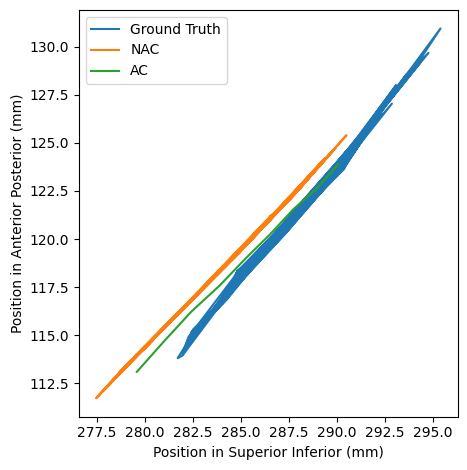
\includegraphics[width=1.0\linewidth]{figures/motion_correction_results_2_com.png}
                
                \captionsetup{singlelinecheck=false, justification=centering}
                \caption{The path of the \gls{COM} of the lesion, in voxel indices. Horizontal (respectively vertical) axis corresponds to motion in the \gls{SI} (respectively \gls{AP}). Different curves denote \gls{COM} displacement for  ground truth data, the estimated data from the \gls{NAC} based \gls{MM} and the estimated data from the \gls{AC} based \gls{MM}.}
                \label{fig:pet_ct_respiratory_motion_correction_with_a_single_attenuation_map_using_nac_derived_deformation_fields_results_com}
            \end{figure}
            
            \gls{COM} results can be seen in~\Fref{fig:pet_ct_respiratory_motion_correction_with_a_single_attenuation_map_using_nac_derived_deformation_fields_results_com}, the \gls{COM} of both the \gls{NAC} and \gls{AC} matches closely the ground truth \gls{COM}.
            
            \begin{figure}
                \centering
                
                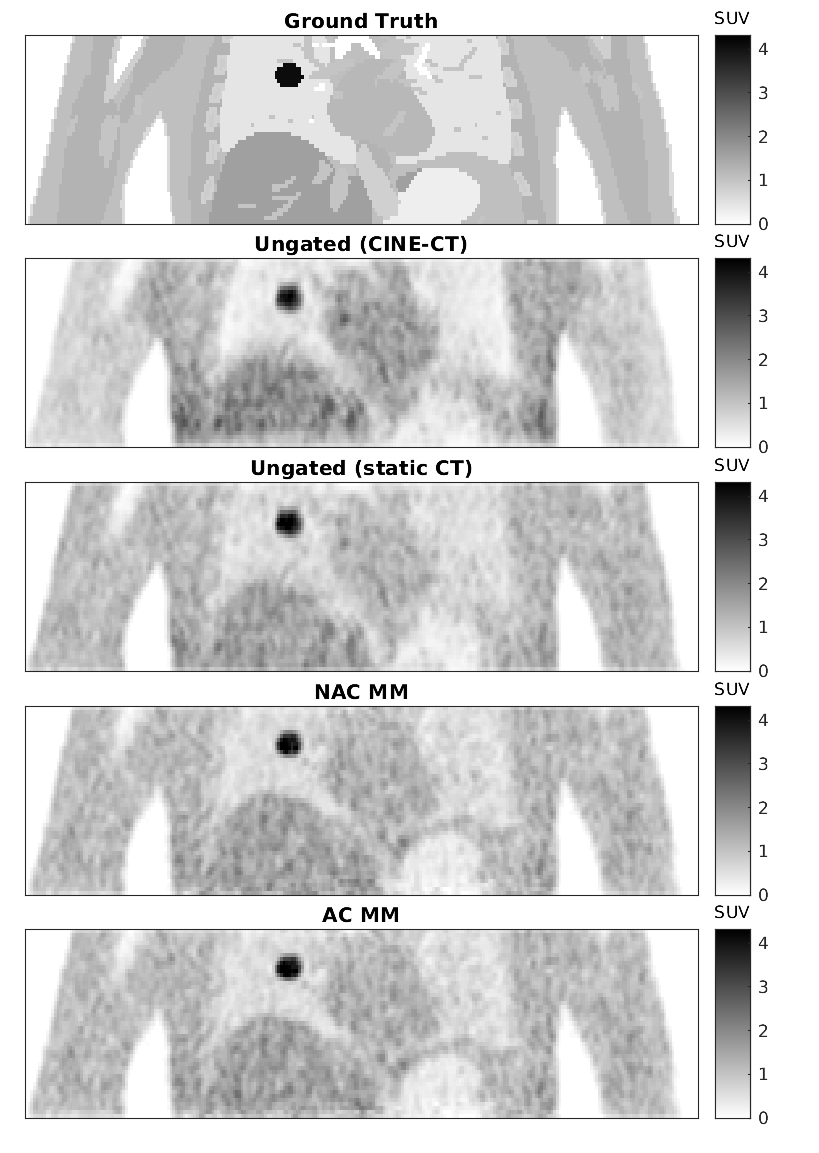
\includegraphics[width=1.0\linewidth]{figures/motion_correction_results_2_visual_analysis.png}
                
                \captionsetup{singlelinecheck=false, justification=centering}
                \caption{Ground truth and reconstructions using; ungated (CINE-\gls{CT}), ungated (static \gls{CT}), \gls{NAC} \gls{MM}, \gls{AC} \gls{MM}. Colour map ranges are consistent for all images.}
                \label{fig:pet_ct_respiratory_motion_correction_with_a_single_attenuation_map_using_nac_derived_deformation_fields_results_visual_analysis}
            \end{figure}
            
            \begin{figure}
                \centering
                
                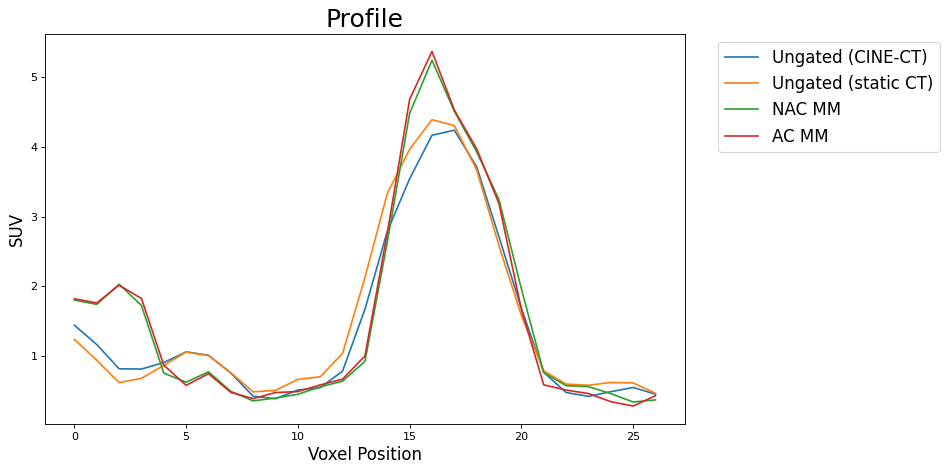
\includegraphics[width=1.0\linewidth]{figures/motion_correction_results_2_profile.png}
                
                \captionsetup{singlelinecheck=false, justification=centering}
                \caption{A profile across the lesion for; ungated (CINE-\gls{CT}), ungated (static \gls{CT}), \gls{NAC} \gls{MM}, \gls{AC} \gls{MM}.}
                \label{fig:pet_ct_respiratory_motion_correction_with_a_single_attenuation_map_using_nac_derived_deformation_fields_results_profile}
            \end{figure}
            
            \begin{table}
                \centering
                
                \captionsetup{singlelinecheck=false, justification=centering}
                \caption{Comparison of \gls{SUV}\textsubscript{max}, \gls{SUV}\textsubscript{median} and \gls{SUV}\textsubscript{peak} between; ungated (CINE-\gls{CT}), ungated (static \gls{CT}), \gls{NAC} \gls{MM}, \gls{AC} \gls{MM}.}
                
                \resizebox*{1.0\linewidth}{!}
                {
                    \begin{tabular}{||c|ccc||}
                        \hline
                        \textbf{\gls{SUV}} & \textbf{Max} & \textbf{Median} & \textbf{Peak} \\
                        \hline
                        \textbf{Ungated (CINE-\gls{CT})}    & $4.63$ & $2.73$ & $3.39$ \\
                        \textbf{Ungated (static \gls{CT})}  & $4.66$ & $3.05$ & $3.54$ \\
                        \hline
                        \textbf{\gls{NAC} \gls{MM}}         & $5.56$ & $3.18$ & $4.07$ \\
                        \textbf{\gls{AC} \gls{MM}}          & $5.43$ & $3.18$ & $4.00$ \\
                        \hline
                    \end{tabular}
                }
                \label{tab:pet_ct_respiratory_motion_correction_with_a_single_attenuation_map_using_nac_derived_deformation_fields_results_suv}
            \end{table}
            
             The ungated and the \gls{MM} data can be seen in~\Fref{fig:pet_ct_respiratory_motion_correction_with_a_single_attenuation_map_using_nac_derived_deformation_fields_results_visual_analysis}. When compared visually structures can be seen, less blurred, in the \gls{MM} data that cannot be seen in the ungated data, for instance, structures at the boundary between the diaphragm and the lung. The different levels of blurring in the ungated (CINE-\gls{CT}) and static \gls{CT} could be attributed to the constraint put on the reconstruction by having a sharp \gls{Mu-Map} in one respiratory position in the static \gls{CT} case. Additionally the lesion itself can be seen to be more homogeneous, this can be observed in the profile across the lesion in~\Fref{fig:pet_ct_respiratory_motion_correction_with_a_single_attenuation_map_using_nac_derived_deformation_fields_results_profile}. \gls{SUV} results can be seen in~\Fref{tab:pet_ct_respiratory_motion_correction_with_a_single_attenuation_map_using_nac_derived_deformation_fields_results_suv} and consistently show that \glss{SUV} are greater for the \gls{MM} over the ungated method.
            
        \subsection{Conclusion} \label{sec:pet_ct_respiratory_motion_correction_with_a_single_attenuation_map_using_nac_derived_deformation_fields_conclusion}
            Results from both a visual analysis, a comparison of profiles and \glss{SUV} show that the \gls{MM} provides volumes more free from blurring and less susceptible to artefacts when compared to the ungated data. Results also indicate that the \gls{NAC} \gls{MM} provides similar volumes while not requiring the additional computation of the \gls{AC} \gls{MM}. Results indicate that \gls{MC} of inter-respiratory cycle motion is possible with this method, while accounting for attenuation deformation.
            
            Future research includes the possibility of directly incorporating the \gls{MM} estimation or estimated \glss{DVF} into the reconstruction algorithm as well as  attempting to simultaneously estimate deformations for the \gls{Mu-Map} as well as the activity distribution. For instance, more complex methods of combining motion estimation and \gls{IR} based on~\boxcite{Bousse2016b} will also be compared. additionally it may also be possible to find better results from improvements to \gls{TOF} resolution~\boxcite{Efthimiou2020UseScanners, Efthimiou2020TOF-PETBGO}. This will be expanded upon in~\Fref{sec:impact_of_tof_on_respiratory_motion_model_estimation_using_nac_pet_discussion}.
    
    \longsection{Comparison of Motion Correction Methods Incorporating Motion Modelling for PET/CT Using a Single Breath Hold Attenuation Map}{sec:comparison_of_motion_correction_methods_incorporating_motion_modelling_for_pet/ct_using_a_single_breath_hold_attenuation_map}
        This section shows a comparison of different \gls{MC} techniques, including with and without incorporating \glss{MM}. The comparison shown here is presented on low count data, so as to better highlight the impact of the addition of \glss{MM}. The \glss{Mu-Map} used are at end inhalation to better reflect clinical breath hold \glss{Mu-Map}.
        
        \subsection{Introduction} \label{sec:comparison_of_motion_correction_methods_incorporating_motion_modelling_for_pet/ct_using_a_single_breath_hold_attenuation_map_introduction}
            \gls{MM} is a \gls{MC} technique, where time- or gate-dependence of \glss{DVF} is parametrised in terms of a \gls{SS}~\boxcite{McClelland2013}. \glss{MM} attempt to improve upon solely registering data, being more robust to noise, but also allowing for the correction of unseen data. It has shown good promise in \gls{CT}~\boxcite{Li2007EnhancedModel}, \gls{MR}~\boxcite{Manke2002RespiratoryModels} and combined \gls{PET}/\gls{MR}~\boxcite{Manber2016JointCorrection.}, but has not yet seen wide spread adoption in clinical \gls{PET}, where \gls{PET}/\gls{CT} is far more common. Respiratory \gls{MC} is an ideal problem area for the application of \glss{MM} as \glss{SS} are already commonly available from respiratory gating, such as acquired by \gls{RPM} or \gls{PCA}~\boxcite{Thielemans2011}.
            
            A method incorporating \glss{MM} for dynamic \gls{PET}/\gls{CT}, was proposed and tested on clinical data in~\boxcite{Chan2018Non-RigidPET}. This work seeks to extend the method, presented in~\Fref{sec:impact_of_tof_on_respiratory_motion_model_estimation_using_pre_gated_no_intra_cycle_motion_nac_pet} and~\Fref{sec:pet_ct_respiratory_motion_correction_with_a_single_attenuation_map_using_nac_derived_deformation_fields}, further through the use of a more modular framework, which allows for the fair comparison of different registration methods, both with and without \glss{MM}. Furthermore, this work uses more realistic simulation and count levels, compared to previous work (where more simple registration methods would fail). Additionally, this work strives to improve the \gls{Mu-Map} warping aspect of previous method, by fixing the \gls{Mu-Map} at end inhalation (as opposed to the mean respiratory position). This is more clinically relevant but also challenging. The work presented here, differentiates itself, specifically from previous work in \gls{MM} for \gls{PET}/\gls{CT}~\boxcite{Chan2018Non-RigidPET}, by firstly using a \gls{2D} \gls{SS}, rather than a \gls{1D} \gls{SS}, thus both inter- and intra-gate motion can be included in the model, at the expense that each gate contains fewer counts. Additionally, the group-wise method, presented here, makes use of an iterative \gls{MC} algorithm rather than using only a pair-wise method.
        
        \section{Methods} \label{sec:comparison_of_motion_correction_methods_incorporating_motion_modelling_for_pet/ct_using_a_single_breath_hold_attenuation_map_methods}
            \subsection{XCAT Volume Generation} \label{sec:comparison_of_motion_correction_methods_incorporating_motion_modelling_for_pet/ct_using_a_single_breath_hold_attenuation_map_xcat_volume_generation}
                Volume generation follows the same basic structure as presented in~\Fref{sec:impact_of_tof_on_respiratory_motion_model_estimation_using_pre_gated_no_intra_cycle_motion_nac_pet_methods_xcat_image_generation} and~\Fref{sec:impact_of_tof_on_respiratory_motion_model_estimation_using_pre_gated_no_intra_cycle_motion_nac_pet_methods_xcat_image_generation}. However the \gls{SS} used to drive \gls{XCAT} was derived from \gls{MR} navigator patient data and a \SI{20}{\milli\metre} diameter spherical lesion (smaller than the max displacement, due to \gls{RM}) was placed into the base of the right lung (within the max displacement, due to \gls{RM}, of the diaphragm).
            
            \subsection{PET Acquisition Simulation and Non-Attenuation Corrected Image Reconstruction} \label{sec:comparison_of_motion_correction_methods_incorporating_motion_modelling_for_pet/ct_using_a_single_breath_hold_attenuation_map_pet_acquisition_simulation_and_non_attenuation_corrected_image_reconstruction}
                Again as in~\Fref{sec:impact_of_tof_on_respiratory_motion_model_estimation_using_pre_gated_no_intra_cycle_motion_nac_pet_methods_pet_data_simulation} and~\Fref{sec:pet_ct_respiratory_motion_correction_with_a_single_attenuation_map_using_nac_derived_deformation_fields_methods_pet_acquisition_simulation} \gls{PET} acquisitions were simulated (and reconstructed) using \gls{STIR}~\boxcite{Thielemans2012}~\boxcite{Nikos2019} through \gls{SIRF}~\boxcite{Ovtchinnikov2017}. Attenuation was included using the relevant \glss{Mu-Map} generated by \gls{XCAT}. Pseudo-randoms and scatter were added. Randoms were added by summing the scaled mean value to each voxel of each volume prior to forward projection. Pseudo scatter was added by summing the scaled and smoothed mean \gls{Mu-Map} prior to forward projection, the smoothing parameter was optimised to give scatter which tapered at the same rate as in clinical data A full scatter simulation was not performed due to software limitations.
                
                Noise was simulated, such that data matched an acquisition over \SI{120}{\second}, emulating a standard single bed position acquisition. The count rate was selected to match that of research scans, i.e. below that of diagnostic clinical scans. This count rate was selected as a 'worst case scenario'.
                
                A respiratory \gls{SS} was generated using \gls{PCA}~\boxcite{Thielemans2011}. The magnitude of this signal and its gradient, was used to gate data into $30$ respiratory bins using displacement gating ($10$ amplitude and $3$ gradient bins). Gates with fewer than $0.42$\% of the counts were discarded. For the purpose of the \gls{MM} fitting, \gls{SS} values were determined for the post-gated data by taking an average of the \gls{SS} values of data in each bin.
                
                Data were reconstructed, without \gls{AC}, using \gls{OSEM} with two full iterations and $24$ subsets~\boxcite{Hudson1994}.
            
            \subsection{Registration} \label{sec:comparison_of_motion_correction_methods_incorporating_motion_modelling_for_pet/ct_using_a_single_breath_hold_attenuation_map_registration}
                Before being registered, each volume underwent pre-processing. Including, replication of end-slices, transformation to be approximately normally distributed~\boxcite{Johnson2013} and post-smoothing. This pre-processing was only applied to intermediate data and was not used for the final output of the method.% Initially, because a breath hold \gls{Mu-Map} is the final target position for the \gls{MC} $10$ repeating slices are added to the top and bottom of each volume to allow space for the volumes to be registered into. First, the mean value was subtracted from each volume and then each voxel in the volume was divided by the standard deviation of the volume. Next a Yeo-Johnson transformation~\boxcite{Johnson2013} was applied to transform data to be more Gaussian like, this acted as a pseudo histogram normalisation. Finally data underwent Gaussian smoothing.
                
                Two registration methods were examined in this work. Firstly, pair-wise registration, where the reference position was selected as the gate with the highest number of counts. All other gates were registered to it. Secondly, group-wise registration, where after an initial pair-wise registration step, the \glss{DVF} generated had the inverse mean of all \glss{DVF} composed with them, before a new reference volume was resampled. Registration to the new reference volume, followed by the inverse mean composition and resample, continued for a set number of iterations. NiftyReg~\boxcite{Modat2010} was used to perform registrations using a B-spline parameterisation. The Gaussian smoothing \gls{FWHM}, \gls{CPG} spacing of the B-spline coefficients, \gls{BE} regularisation term weight and number of iterations were tuned using a grid search.
            
            \subsection{Motion Model Estimation} \label{sec:comparison_of_motion_correction_methods_incorporating_motion_modelling_for_pet/ct_using_a_single_breath_hold_attenuation_map_motion_model_estimation}
                If a \gls{MM} was used, then it was fit as a direct \gls{RCM} on the \glss{DVF} from~\Fref{sec:comparison_of_motion_correction_methods_incorporating_motion_modelling_for_pet/ct_using_a_single_breath_hold_attenuation_map_registration} and the \gls{SS} from~\Fref{sec:comparison_of_motion_correction_methods_incorporating_motion_modelling_for_pet/ct_using_a_single_breath_hold_attenuation_map_pet_acquisition_simulation_and_non_attenuation_corrected_image_reconstruction}. A weighted \gls{LR} was used, where the weighting was taken based on the number of counts in each gate. Once a \gls{MM} was fit, new \glss{DVF} were generated for each gate, using the \gls{SS} values used to fit the \gls{MM}. For group-wise registration, \gls{MM} fitting occurred between iterations, the \glss{DVF} generated by the \gls{MM} were used to resample the new target volume at each iteration.
            
            \subsection{Attenuation Map Warping} \label{sec:comparison_of_motion_correction_methods_incorporating_motion_modelling_for_pet/ct_using_a_single_breath_hold_attenuation_map_attenuation_map_warping}
                A \gls{Mu-Map} at end inhalation was selected from the \glss{Mu-Map} generated by \gls{XCAT}. The \gls{PET} volume from the previous step was then registered to this \gls{Mu-Map}, and the resulting \glss{DVF} were composed with the \glss{DVF} from the last iteration of the \gls{MC} method, and a new volume resampled. The inverse of these \glss{DVF}, were then used to warp the \gls{Mu-Map} to each gate.
            
            \subsection{Motion Corrected Image Reconstruction with AC} \label{sec:comparison_of_motion_correction_methods_incorporating_motion_modelling_for_pet/ct_using_a_single_breath_hold_attenuation_map_attenuation_corrected_image_reconstruction}
                Data were re-reconstructed with \gls{AC}, using the \glss{Mu-Map} from~\Fref{sec:comparison_of_motion_correction_methods_incorporating_motion_modelling_for_pet/ct_using_a_single_breath_hold_attenuation_map_attenuation_map_warping}. The same reconstruction parameters as in~\Fref{sec:comparison_of_motion_correction_methods_incorporating_motion_modelling_for_pet/ct_using_a_single_breath_hold_attenuation_map_attenuation_corrected_image_reconstruction} were used. \gls{MC} was then applied to data following~\Fref{sec:comparison_of_motion_correction_methods_incorporating_motion_modelling_for_pet/ct_using_a_single_breath_hold_attenuation_map_registration},~\Fref{sec:comparison_of_motion_correction_methods_incorporating_motion_modelling_for_pet/ct_using_a_single_breath_hold_attenuation_map_motion_model_estimation} and~\Fref{sec:comparison_of_motion_correction_methods_incorporating_motion_modelling_for_pet/ct_using_a_single_breath_hold_attenuation_map_attenuation_map_warping}. Volumes were post-filtered using a Gaussian smoothing, with a \gls{FWHM} of \SI{6.39}{\milli\metre} in the transverse plane (equivalent to three voxels) and \SI{3.27}{\milli\metre} (equivalent to one voxel) in the axial direction.
            
            \subsection{Evaluation} \label{sec:comparison_of_motion_correction_methods_incorporating_motion_modelling_for_pet/ct_using_a_single_breath_hold_attenuation_map_evaluation}
                In addition to the reconstructions performed in~\Fref{sec:comparison_of_motion_correction_methods_incorporating_motion_modelling_for_pet/ct_using_a_single_breath_hold_attenuation_map_attenuation_corrected_image_reconstruction}, data were also reconstructed without \gls{MC}, using either a sum of all \glss{Mu-Map} (to emulate an \gls{AV-CCT}), or the end inhalation \gls{Mu-Map}. For the present evaluation, the volumes without \gls{MC} were registered to the position of the end inhalation \gls{Mu-Map}. Additionally, \glss{DVF} generated by each method were also applied to noiseless data for visual analysis.
                
                Comparisons used included: A profile over the lesion, \gls{SUV}\textsubscript{max} and \gls{SUV}\textsubscript{peak} (defined following \gls{EANM} guidelines~\boxcite{Boellaard2015FDG2.0}).
        
        \section{Results} \label{sec:comparison_of_motion_correction_methods_incorporating_motion_modelling_for_pet/ct_using_a_single_breath_hold_attenuation_map_results}
            \begin{figure}
                \centering
                
                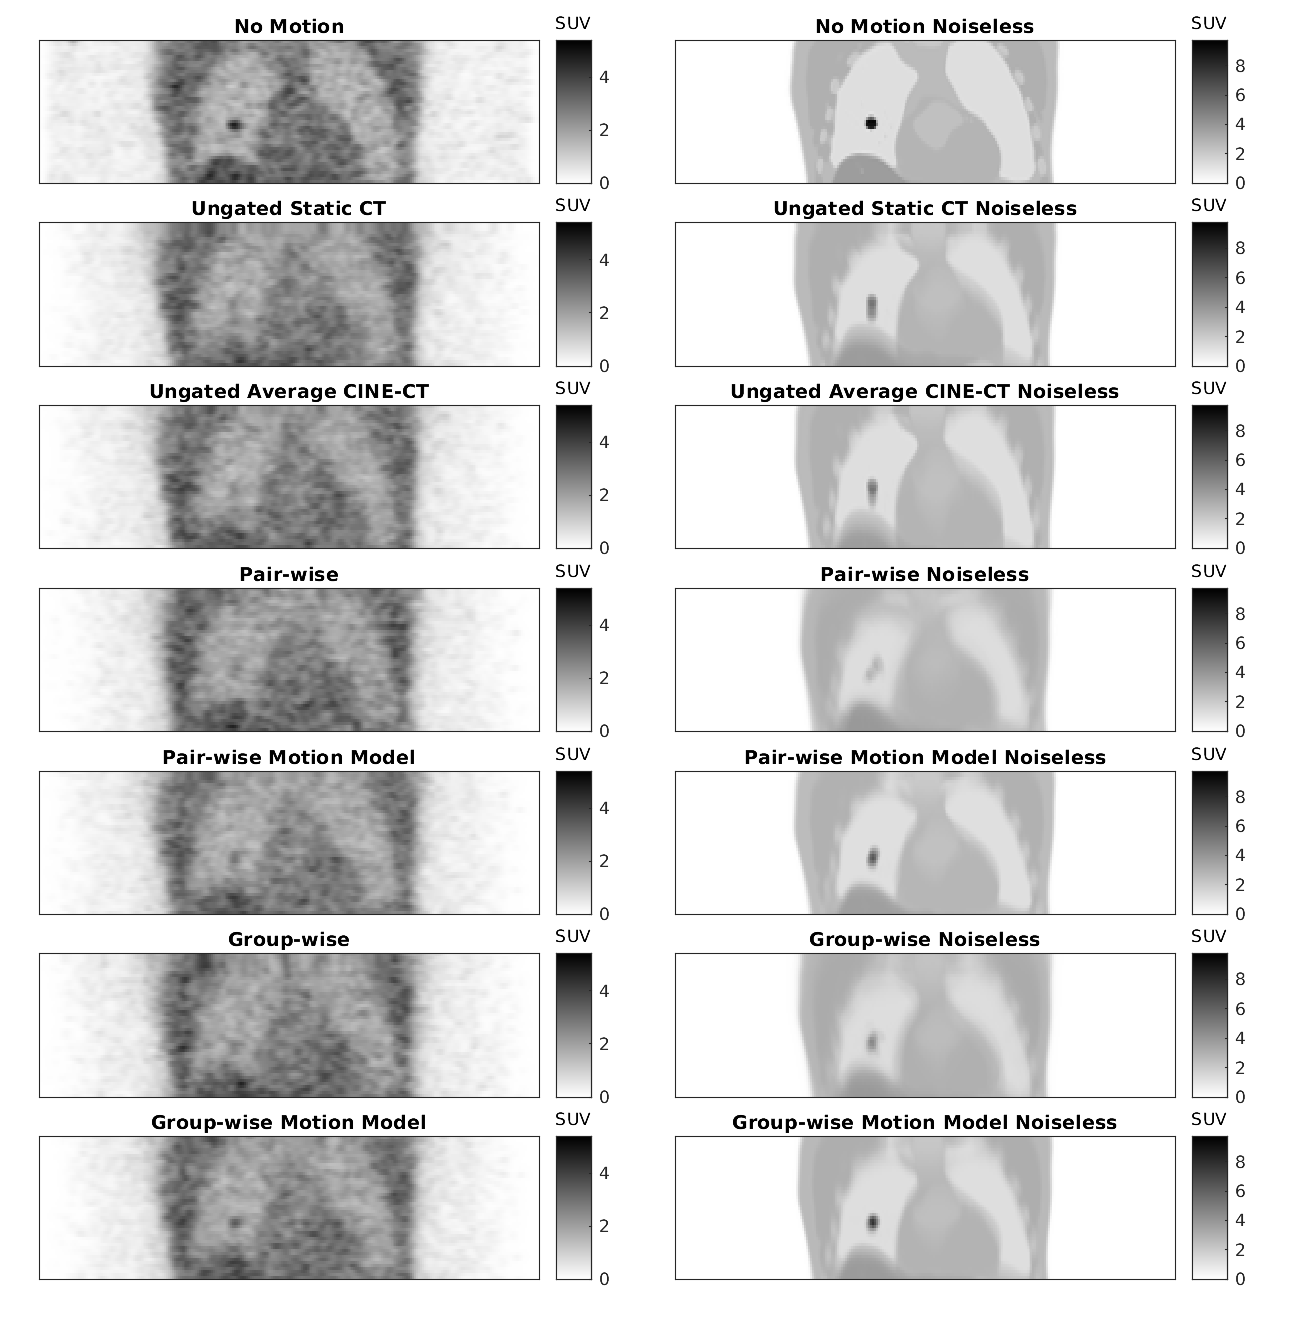
\includegraphics[width=1.0\linewidth]{figures/motion_correction_results_3_visual_analysis.png}
                
                \captionsetup{singlelinecheck=false, justification=centering}
                \caption{First column contains \gls{AC} \gls{MC} reconstructions and the second column contains the result of applying the final  \gls{MC} on the original XCAT images (for easier assessment of the accuracy of the estimated \glss{DVF}); ungated static \gls{CT}, ungated \gls{AV-CCT}, pair-wise, pair-wise \gls{MM}, group-wise, group-wise \gls{MM}. Colour map ranges are consistent for all images in each column.}
                \label{fig:comparison_of_motion_correction_methods_incorporating_motion_modelling_for_pet/ct_using_a_single_breath_hold_attenuation_map_visual_analysis}
            \end{figure}
            
            \begin{figure}
                \centering
                
                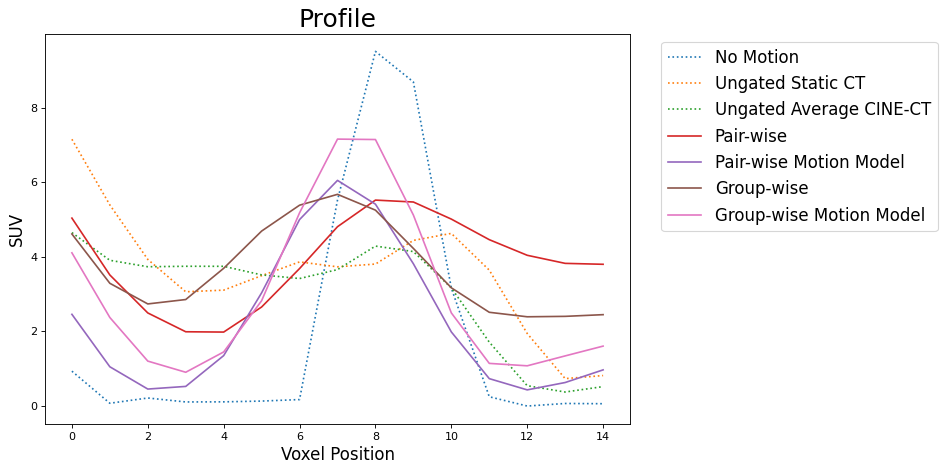
\includegraphics[width=1.0\linewidth]{figures/motion_correction_results_3_profile.png}
                
                \captionsetup{singlelinecheck=false, justification=centering}
                \caption{A profile across the lesion for; ungated static \gls{CT}, ungated \gls{AV-CCT}, pair-wise, pair-wise \gls{MM}, group-wise, group-wise \gls{MM}.}
                \label{fig:comparison_of_motion_correction_methods_incorporating_motion_modelling_for_pet/ct_using_a_single_breath_hold_attenuation_map_profile}
            \end{figure}
            
            \begin{table}
                \centering
                
                \captionsetup{singlelinecheck=false, justification=centering}
                \caption{Comparison of \gls{SUV}\textsubscript{max} and \gls{SUV}\textsubscript{peak} between: ungated static \gls{CT}, ungated \gls{AV-CCT}, pair-wise, pair-wise \gls{MM}, group-wise, group-wise \gls{MM}.}
                
                \resizebox*{1.0\linewidth}{!}
                {
                    \begin{tabular}{||c|cc||}
                        \hline
                        \textbf{\gls{SUV}}                  & \textbf{Max}  & \textbf{Peak} \\
                        \hline
                        \textbf{No Motion}                  & $9.50$        & $9.06$ \\
                        \hline
                        \textbf{Ungated Static \gls{CT}}    & $5.25$        & $5.15$ \\
                        \textbf{Ungated \gls{AV-CCT}}       & $5.38$        & $5.07$ \\
                        \hline
                        \textbf{Pair-wise}                  & $4.21$        & $3.92$ \\
                        \textbf{Pair-wise \gls{MM}}         & $6.63$        & $6.07$ \\
                        \hline
                        \textbf{Group-wise}                 & $4.42$        & $4.21$ \\
                        \textbf{Group-wise \gls{MM}}        & $7.64$        & $7.03$ \\
                        \hline
                    \end{tabular}
                }
                \label{tab:comparison_of_motion_correction_methods_incorporating_motion_modelling_for_pet/ct_using_a_single_breath_hold_attenuation_map_suv}
            \end{table}
            
            A visual comparison of the reconstructed images (see ~\Fref{fig:comparison_of_motion_correction_methods_incorporating_motion_modelling_for_pet/ct_using_a_single_breath_hold_attenuation_map_visual_analysis}), shows that more blurring can be seen at the boundary between the diaphragm and lung for the \gls{MM}-free methods. Additionally, where a \gls{MM} was used, the lesion appears to be more homogeneous.
             
            The peak of the profile (see~\Fref{fig:comparison_of_motion_correction_methods_incorporating_motion_modelling_for_pet/ct_using_a_single_breath_hold_attenuation_map_profile}), is greater for \gls{MM} methods than for \gls{MM}-free methods. However, the peak for all \gls{MC} methods are greater than ungated methods.
             
            \gls{SUV} results consistently show that including \glss{MM} increases the \gls{SUV} when compared to when one is not used (see~\Fref{tab:comparison_of_motion_correction_methods_incorporating_motion_modelling_for_pet/ct_using_a_single_breath_hold_attenuation_map_suv}).
        
        \section{Conclusion} \label{sec:comparison_of_motion_correction_methods_incorporating_motion_modelling_for_pet/ct_using_a_single_breath_hold_attenuation_map_conclusions}
            Results from a visual analysis, a comparison of profiles and \gls{SUV}, show that adding a \gls{MM} to any \gls{MC} method (tested here) improved the quality of volumes produced. Although, from a visual analysis volumes appear preferable with any \gls{MC} method, quantitative evaluation points to the conclusion that for \gls{MC} to be successful, for very noisy data, \glss{MM} are almost required.
            
            In the future, work will focus on incorporating the methods presented here into an iterative \gls{PET} reconstruction and \gls{MC} method and tested on patient data from several research studies. It may also be of interest to consider the impact that robust regression methods have on fitting a \gls{MM}, such as using a robust objective function or fitting the \gls{MM} indirectly on the eigenvectors of applying \gls{PCA} to the initial \glss{DVF}.
    
    \longsection{Discussion}{sec:impact_of_tof_on_respiratory_motion_model_estimation_using_nac_pet_discussion}
        The methods presented above suffer from a number of issues which future work will seek to rectify. Firstly, an obvious hole in the results presented above is that the method has only been tested on simulated data. Thus, it cannot be said that if the method works here that it can be extrapolated that it also works on clinical data. For instance, the initial activity distributions are taken from \gls{XCAT} simulated volumes, these volumes suffer from the fact that within a feature they are almost entirely homogeneous. If the intensity of the activity volume were examined the intensity within an organ or tissue would almost never vary. This actually poses a significant problem to most registration algorithms, where there would be no gradient across a homogeneous region thus the reconstruction is more likely to terminate early with a poor result or otherwise be unable to find a good direction to update in.
        
        An additional issue posed by the use of \gls{XCAT} simulations would be that the \gls{MM} used to drive the simulation over time is rather simple, it is a linear \gls{MM}. This means that for a given value of the \gls{SS} the anatomy will always be in the same place. Whereas, a patient is more likely to have breath to breath variability and the motion present will almost never be able to be entirely represented by a linear system. The \gls{MM} method used in the work above also uses a linear \gls{MM}, meaning that all of the motion present in the data could be captured unadulterated by the method (under ideal circumstances) possibly giving misleading results. The fact that the \gls{MM} used is linear in and of itself could be a limitation, a patient is unlikely to breath following a linear model. As such when it is possible to test the method using data generated using a non-linear model, it could be advantageous to also incorporate a non-linear model into the \gls{MM}.
        
        Furthermore, the \gls{SS} used during the \gls{XCAT} simulation, for most of this work, is identical (but flipped) for both the \gls{AP} and \gls{SI} motion. This means that there is no hysteresis in the motion, which is unrealistic. This could be solved by giving separate signals (a \gls{2D} signal) for both the \gls{AP} and \gls{SI} motion, which are captured using an \gls{MR} scanner, rather than a \gls{1D} signal captured from an \gls{RPM}. This has begun to be addressed by using an \gls{MR} derived signal in~\Fref{sec:comparison_of_motion_correction_methods_incorporating_motion_modelling_for_pet/ct_using_a_single_breath_hold_attenuation_map}.
        
        The anatomy used for the \gls{XCAT} simulation did not vary, it was an average male anatomy. In order to prove generalisability, and to avoid unnecessary bias, ideally the method would be tested on a multitude of anatomy including both male and female, big and small. This is compounded by the fact that the lesion used to demonstrate the improvement by the \gls{MC} method was unreasonably large, \gls{MC} wouldn't be needed to identify and locate it. In order to better highlight the advantage of the \gls{MC} method a smaller lesion placed closer to the diaphragm should be used. This also has begun to be addressed in~\Fref{sec:comparison_of_motion_correction_methods_incorporating_motion_modelling_for_pet/ct_using_a_single_breath_hold_attenuation_map}.
        
        Although \gls{18F-FDG} is the most commonly used radiotracer, it isn't the only used radiotracer. If this method were used during cardiac imaging it most likely wouldn't be the tracer used. Given this, the activity values used during the \gls{XCAT} simulation were taken from a clinical \gls{18F-FDG} scan and as such the method hasn't been tested in these circumstances.
        
        The method to simulate the \gls{PET} acquisition also has some limitations. Firstly, in the work presented here a relatively high count rate is used for the noise caused by the \gls{PET} acquisition physics. It may be interesting to look at how the \gls{MC} methods perform under more strenuous circumstance, for instance, research scan count rate levels. Additionally, as mentioned above in both~\Fref{sec:impact_of_tof_on_respiratory_motion_model_estimation_using_pre_gated_no_intra_cycle_motion_nac_pet_methods_pet_data_simulation} and~\Fref{sec:pet_ct_respiratory_motion_correction_with_a_single_attenuation_map_using_nac_derived_deformation_fields_methods_pet_acquisition_simulation} no random or scatter simulation were used. This is clearly unrealistic as a \gls{PET} scan could never take place without either random or scatter events, even if they were corrected for. The reason for a lack of random or scatter simulation was because the software available did not provide this functionality when using \gls{TOF} simulations. This has begun to be addressed in~\Fref{sec:comparison_of_motion_correction_methods_incorporating_motion_modelling_for_pet/ct_using_a_single_breath_hold_attenuation_map}. This is being addressed using a lower count simulation and also by including pseudo-random and scatter.
        
        \gls{TOF} resolutions used in the work are not reflected in any current scanner. The \gls{TOF} resolution in conjunction with the voxel size were chosen as a compromise between two current systems to give the method the best chance of working. However, obviously this means there is no clinical data available to test the method on that wouldn't also mean changing one of either the \gls{TOF} resolution or the voxel size. If the \gls{GE} Discovery $710$ were selected to perform scans to test this method it would also mean sacrificing some \gls{TOF} resolution.
        
        Building from the limitations highlighted in the \gls{MC} and \gls{MM} earlier, the registrations performed as part of the \gls{MM} were fit using \gls{SSD}. This objective function is sensitive to differences in the magnitude of the input. If gates are registered to a mean volume, as in group-wise registration seen earlier in~\Fref{sec:applying_image_registration}, then the magnitude of the inputs will never be equal. Additionally, if \gls{SSD} were used to register a \gls{PET} activity distribution to a \gls{CT} \gls{Mu-Map} it would also fail for the same reasons. This problem could be solved by preprocessing the data, however, it could also be addressed by changing the objective function to something such as \gls{NMI}. This has begun to be addressed in~\Fref{sec:comparison_of_motion_correction_methods_incorporating_motion_modelling_for_pet/ct_using_a_single_breath_hold_attenuation_map}. Here \gls{NMI} was included, however this the method used did not fit the \gls{MC} and \gls{MM} simultaneously.
        
        Furthermore, the objective function used for the \gls{MM} fitting also used \gls{SSD} which is sensitive to outliers. This would cause a limitation during early iterations of the \gls{MC} when it is likely that the quality of the registration is poor and thus the B-spline coefficients or the \gls{DVF} is also poor. This limitation may be compounded if the method were combined, as is, iteratively with \gls{PET} reconstruction. This is because, at early time points not only would the registration be poor but the volumes provided to the registration by the reconstruction would also be poor. To mitigate this an objective function which is robust to outliers could be used, such as Huber. Huber is defined as being equivalent to squared error below a threshold and absolute error above it.
        
        A final limitation and a possible future direction for research would be that the objective function for the registration is currently calculated in image space. If the objective function were shifted to sinogram space then it would be much more likely that a combined iterative \gls{PET} reconstruction and \gls{MC} would converge to a good solution due to the fact that both methods are using objective functions calculated in the same space.
